\chapter{Estimation Based on Normal Distribution}

\section{Point Estimation of Mean and Variance}
\subsection{Introduction}
Assume that some characteristics of the elements in a population can be represented by a random variable $X$ whose p.d.f. (or p.f.) is $f_X(x; \theta)$, where the form of the probability density function (or probability function) is assumed known except that it contains an unknown parameter $\theta$. \\
Further assume that the values $x_1, x_2, \dots, x_n$ of a random sample $X_1, X_2, \dots, X_n$ from $f_X(x; \theta)$ can be observed. On the basis of the observed sample values $x_1, x_2, \dots, x_n,$, it is desired to estimate the value of the unknown parameter $\theta$.

\subsection{Estimation}
The estimation can be made in 2 ways: \textbf{Point estimation} and \textbf{Interval estimation}. \\
Point estimation is to let the value of some statistic, say
$$
\hat{\Theta} = \hat{\Theta}(X_1, X_2, \dots, X_n),
$$
to estimate the unknown parameters $\theta$. \\
Such a statistic $\hat{\Theta}(X_1, X_2, \dots, X_n)$ is called a \textbf{point estimator}.\\
Recall that a statistic is a function of the random sample which does not depend on any unknown parameters. Examples of statistic include $\bar{X} = \dfrac{1}{n} \sum_{i = 1}^n X_i$ or $X_{(n)} = max(X_1, X_2, \dots, X_n)$. \\
Let $W = \dfrac{1}{n} \sum_{i = 1}^n (X_i - \mu)^2$. Then $W$ is not a statistic if $\mu$ is not known. However, $W$ is a statistic if $\mu$ is known.

\subsection{Point Estimate of Mean}
Suppose $\mu$ is the population mean. The statistic that one uses to obtain a point estimate is called an estimator. For example, $\bar{X}$ is an estimator of $\mu$. The value of $\bar{X}$, denoted by $\bar{x}$, is an estimate of $\mu$. \\
It should not come as a surprise that different random samples give different point estimates of $\mu$.
\begin{note}
\end{note}
It is important to distinguish clearly these three concepts: an estimator/statistic (e.g. $\bar{X}$), an estimate (e.g. $\bar{x}$), and a population parameter (e.g.$\mu$). An estimator/statistic is a computational rule. It is also a random variable. When the data (random sample) are available, it tells us how to compute. An estimate is a computed value of the estimator based on the observed data (random sample). It is not a random variable - it is a particular realization of the random variable. A population parameter is something about the population - it is not a random variable. Even if you do not know the population parameter, it is an unknown constant, NOT a random variable.

\subsection{Interval Estimation}
Interval estimation is to define two statistics, say, $\hat{\Theta_L}$ and $\hat{\Theta_U}$, where $\hat{\Theta_L} < \hat{\Theta_U}$ so that $(\hat{\Theta_L},\hat{\Theta_U})$ constitutes a random interval for which the probability of containing the unknown parameter $\theta$ can be determined. \\
For example, suppose $\sigma^2$ is known. Let
$$
\hat{\Theta_L} = \bar{X} - 2 \dfrac{\sigma}{\sqrt{n}} \textit{ and } \hat{\Theta_R} = \bar{X} + 2 \dfrac{\sigma}{\sqrt{n}}
$$
Then, $\left(\bar{X} - 2 \dfrac{\sigma}{\sqrt{n}}, \bar{X} + 2 \dfrac{\sigma}{\sqrt{n}} \right)$ is an interval estimator for $\mu$. 
\subsection{Biased and Unbiased Estimators}
\begin{definition}[Unbiased estimator]
A statistic $\hat{\Theta}$ is said to be an unbiased estimator of the parameter $\theta$ if $E[\hat{\Theta}] = \theta$.
\end{definition}
For example, $\bar{X}$ is an unbiased estimator of $\mu$. That is, $E[\bar{X}] = \mu$. \\
Also, $S^2 = \dfrac{1}{n - 1}\sum_{i = 1}^n (X_i - \bar{X})^2$ is an unbiased estimator of $\sigma^2$. That is, $E[S^2] = \sigma^2$. \\
However, $T = \dfrac{1}{n}\sum_{i = 1}^n (X_i - \bar{X})^2$ is a \textbf{biased} estimator of $\sigma^2$.  It can be shown that $E[T] = \dfrac{n-1}{n}\sigma^2 \neq \sigma^2$
\begin{note}
\end{note}
Here is a short derivation for $E[S^2] = \sigma^2$:
\begin{equation*}
    \begin{split}
        \sum_{i = 1}^n (X_i - \bar{X})^2 &= \sum_{i = 1}^n (X_i^2 - 2\bar{X}X_i + \bar{X}^2) \\
        &= \sum_{i = 1}^n X_i^2 - 2 \bar{X} \sum_{i = 1}^n X_i + n\bar{X}^2 \\
        &= \sum_{i = 1}^n X_i^2 - 2n\bar{X}^2 + n\bar{X}^2 \textit{ (because } \bar{X} = \dfrac{\sum_{i = 1}^n X_i}{n} \textit{ )} \\
        &= \sum_{i = 1}^n X_i^2  - n\bar{X}^2 \\
        Now,
        E[S^2] &= E\left[\dfrac{1}{n - 1} \sum_{i = 1}^n (X_i - \bar{X})^2\right] \\
        &= \dfrac{1}{n - 1} E\left[ \sum_{i = 1}^n X_i^2 - n\bar{X}^2\right] \textit{ (based on the result above)} \\
        &= \dfrac{1}{n - 1}\left( E\left[ \sum_{i = 1}^n X_i^2 \right] - n E[\bar{X}^2]\right) \textit{ (linearity of expectation)}\\
        &= \dfrac{1}{n - 1}  \left(\sum_{i = 1}^n E[X_i^2]  - n E[\bar{X}^2] \right) \textit{ (linearity of expectation)} \\
        &= \dfrac{1}{n - 1} \left( \sum_{i = 1}^n[V(X_i) + (E[X])^2] - n[V(\bar{X}) + (E[\bar{X}])^2] \right) \textit{ (because } V(Y) = E[Y^2] - (E[Y])^2 \textit{ )}\\
        &= \dfrac{1}{n - 1} \left ( n \sigma^2 + n\mu^2 - \sigma^2 - n\mu^2 \right ) \textit{ (because } E[X] = \mu, V(X) = \sigma^2, E[\bar{X}] = \mu, V(\bar{X}) = \dfrac{\sigma^2}{n} \textit{ )}\\
        &= \dfrac{1}{n - 1} (n - 1)\sigma^2 \\
        &= \sigma^2
    \end{split}
\end{equation*}
\begin{note}
\end{note}
Let $X_1, X_2, \dots, X_n$ be a random sample. Then, observe that $E(X_1) = \mu$, i.e., $X_1$ is also an unbiased estimator for $\mu$. So, why do we bother to use $\bar{X}$ instead of simply using $X_1$? \\
The answer is quite simple. The variance of $X_1$ is $\sigma^2$. The variance of $\bar{X}$ is $\frac{\sigma^2}{n}$ where $n$ is the sample size. This means that $\bar{X}$ varies less than $X_1$ and so it makes more sense to use that to estimate the population mean. This also provides some intuition as to why the variance of $\bar{X}$ is $\dfrac{\sigma^2}{n}$. We know that $\mu$ is a constant and has variance = 0. So, the larger the sample size, the better the estimate (closer to constant $\mu$) and hence, lower the variability. We're taking the mean of $n$ random variables and so, the variation reduces too.
\begin{note}
\end{note}
Our aim is to find an estimator which is unbiased and has a low variance. But even if a biased estimator has a very low variance, it is not a good estimator. Being unbiased matters more than having low variance. Accuracy (how close your estimate is to the actual value) is more important than precision (how close your estimates are to each other). Consistency matters only when you're actually estimating well. In practice, we choose the estimator with the lowest MSE (Mean Square Error) - We try to minimize the mean of the squares of the error between our estimate and the actual value. For an unbiased estimator, the MSE = variance.
\section{Interval Estimation}
An interval estimate of a population parameter $\theta$ is an interval of the form $\hat{\theta_L} < \theta < \hat{\theta_U}$, where $\hat{\theta_L}$ and $\hat{\theta_U}$ depend on 
\begin{enumerate}
    \item The value of the statistic $\hat{\Theta}$ for the particular sample, and
    \item The sampling distribution of $\hat{\Theta}$
\end{enumerate}
\begin{figure}
    \centering
    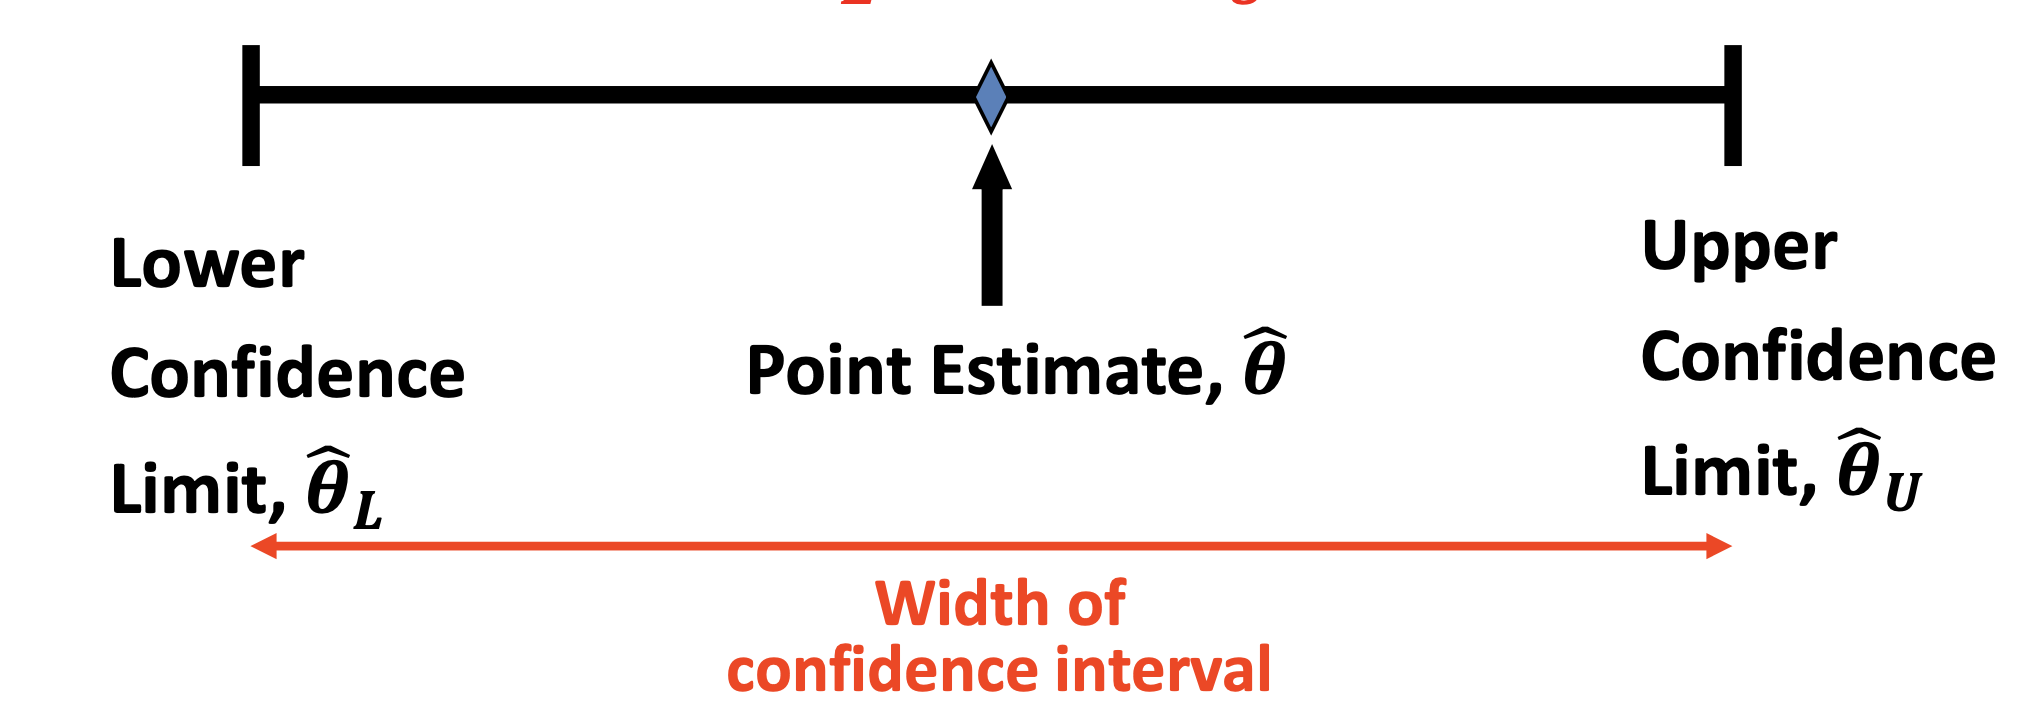
\includegraphics[width = 15cm]{Images/Interval estimation.png}
    \caption{Interval Estimation}
    \label{fig:my_label}
\end{figure}
Since different samples will generally yield different values of $\hat{\Theta}$, and therefore different values of $\hat{\theta_L}$ and $\hat{\theta_U}$, these end points of the interval are values of corresponding random variables $\hat{\Theta_L}$ and $\hat{\Theta_U}$. \\
These intervals may not contain the parameter $\theta$ as $\hat{\theta_L}$ and $\hat{\theta_U}$ vary. \\
We shall seek a random interval $(\hat{\Theta_L}, \hat{\Theta_U})$ containing $\theta$ with a given probability $1 - \alpha$. That is, $P(\hat{\Theta_L} < \theta < \hat{\Theta_U}) = 1 - \alpha$. Then the interval $\hat{\theta_L} < \theta < \hat{\theta_U}$ computed from the selected sample is called a $(1 - \alpha)100\%$ confidence interval for $\theta$ and the fraction $(1 - \alpha)$ is called the \textbf{confidence coefficient} or \textbf{degree of confidence}, and the endpoints $\hat{\theta_L}$ and $\hat{\theta_U}$ are called the lower and upper confidence limits respectively. \\
This means that if samples of the same size $n$ are taken, then in the long run, $(1 - \alpha)100\%$ of the intervals will contain the unknown parameter $\theta$, and hence with a confidence of $(1 - \alpha)100\%$, we can say that the interval covers $\theta$.
\begin{figure}
    \centering
    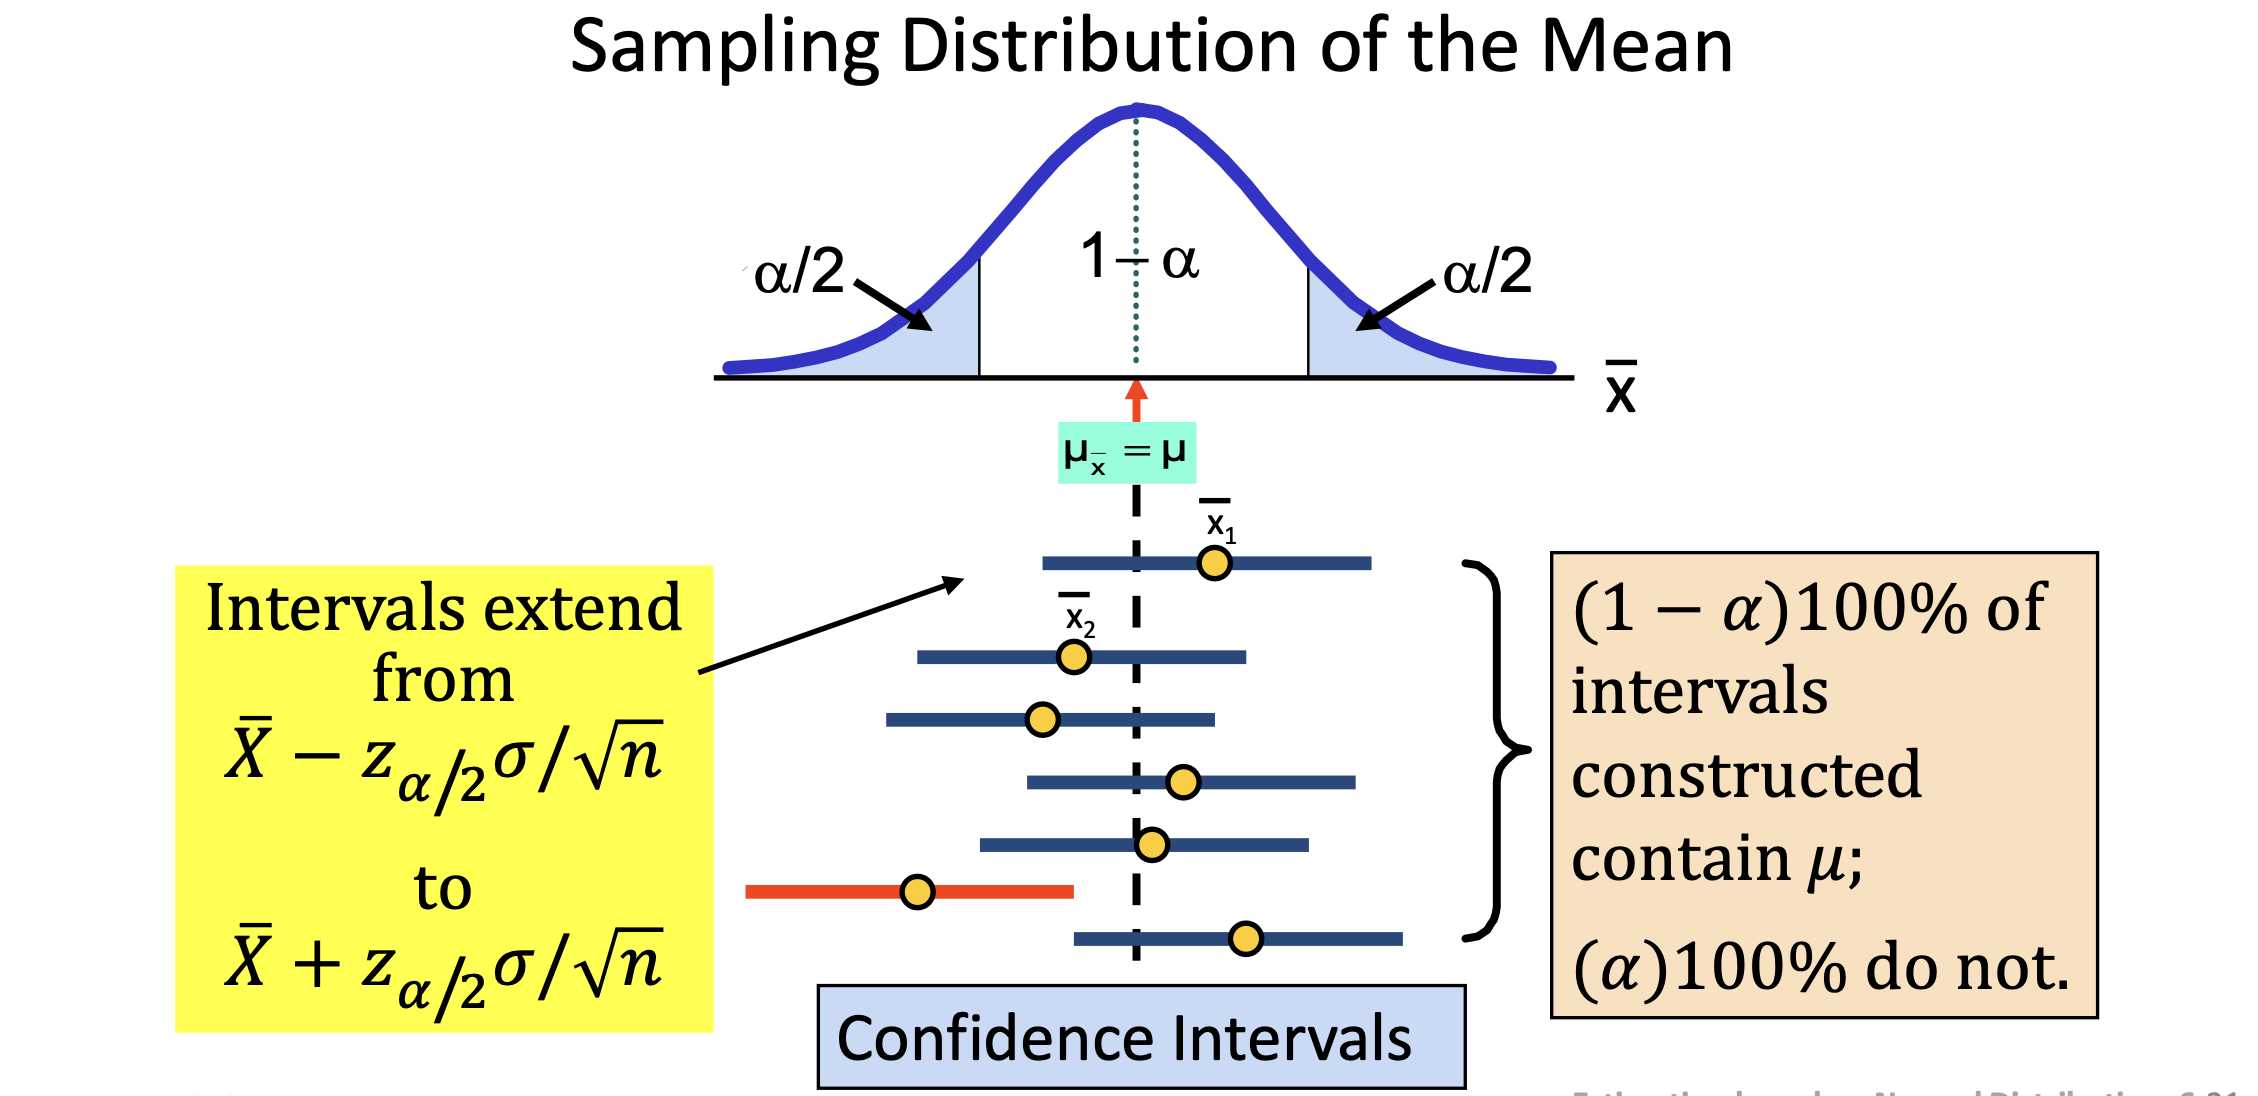
\includegraphics[width = 15cm]{Images/Sampling Distribution of the Mean.png}
    \caption{Sampling Distribution of the Mean}
    \label{fig:my_label}
\end{figure}
\begin{note}
\end{note}
It is important to differentiate the random interval from the interval estimate. Once you have realized the values of the upper and lower bounds of the interval, it does not make sense to talk about the probability of a population parameter lying within the interval. The population parameter is an unknown constant. It either does or does not lie within the computed interval - there is no notion of probability involved. Practically, for a computed C.I., we can only claim that with a certain confidence the interval will cover the true value. This is the reason we choose to say "confidence" rather than "probability"
\section{Confidence Interval (C.I.) for the Mean}
\subsection{Known Variance Case}
Assume that we know the population variance and we are trying to estimate the population mean. Further, we also know that the population distribution is normal or $n$ is sufficiently large (say $n \geq 30)$. \\
Then, by the Central Limit Theorem, we can expect that $\bar{X} \sim N\left(\mu, \dfrac{\sigma^2}{n}\right)$. Therefore, $Z = \dfrac{\bar{X} - \mu }{\sigma/\sqrt{n}} \sim N(0,1)$. Hence,
$$
P\left(-z_{\alpha/2} < \dfrac{\bar{X} - \mu }{\sigma/\sqrt{n}} < z_{\alpha/2}\right) = 1 - \alpha
$$ or
$$
P\left( \bar{X} - z_{\alpha/2}\dfrac{\sigma}{\sqrt{n}} < \mu < \bar{X} + z_{\alpha/2}\dfrac{\sigma}{\sqrt{n}} \right ) = 1 - \alpha
$$
Recall that $P(Z \geq z_{\alpha}) = \alpha$ as per our definition of $z_{\alpha}$. \\
\imp{
Hence, if $\bar{X}$ is the mean of a random sample of size $n$ from a population with known variance $\sigma^2$, a $(1 - \alpha)100\%$ confidence interval for $\mu$ is given by 
$$
\left (\bar{X} - z_{\alpha/2}\dfrac{\sigma}{\sqrt{n}} < \mu < \bar{X} + z_{\alpha/2}\dfrac{\sigma}{\sqrt{n}} \right )
$$}
\subsection{Sampling Size for Estimating $\mu$}
Most of the time, $\bar{X}$ will not be exactly equal to $\mu$ and the point estimate is in error. The size of this error will be $| \bar{x} - \mu |$. We know that 
$P\left( \bar{X} - z_{\alpha/2}\dfrac{\sigma}{\sqrt{n}} < \mu < \bar{X} + z_{\alpha/2}\dfrac{\sigma}{\sqrt{n}} \right ) = 1 - \alpha$. In other words, 
$$
P\left( |\bar{X} - \mu | < z_{\alpha/2} \dfrac{\sigma}{\sqrt{n}}\right) = 1 - \alpha
$$
Let $e$ denote the margin of error. We want the error $|\bar{X} - \mu |$ does not exceed the margin of error, $e$, with a probability larger than $1 - \alpha$. That is,
$$
P(|\bar{X} - \mu | \leq e) \geq 1 - \alpha
$$
Since $P\left( |\bar{X} - \mu | < z_{\alpha/2} \dfrac{\sigma}{\sqrt{n}}\right) = 1 - \alpha$, therefore
$$
e \geq z_{\alpha/2} \dfrac{\sigma}{\sqrt{n}}
$$
Hence for a given margin of error $e$, the sample size is given by
\imp{
$$
n \geq \left( z_{\alpha/2}\dfrac{\sigma}{e} \right)^2
$$}
\begin{note}
\end{note}
It is important to understand the implications of the above formula. The required sample size depends on:
\begin{enumerate}
    \item $z_{\alpha/2}$ (and hence on $\alpha$). In particular, lower the value of $\alpha$, higher the value of $z_{\alpha/2}$. So, for a higher degree of confidence, we need to have a larger sample size (as expected)
    \item $\sigma$ - If the underlying distribution shows higher variation, it is necessary to have a larger sample size to have the same margin of error and degree of confidence.
    \item $e$ - To have a lower margin of error, you need to have a higher sample size.
\end{enumerate}
\subsection{Unknown Variance Case}
We now try to find the confidence interval for mean with:
\begin{enumerate}
    \item unknown population variance
    \item the population is normal or very close to normal distribution
    \item the sample size is small (so we cannot use central limit theorem)
\end{enumerate}
Let $T = \dfrac{\bar{X} - \mu }{S/\sqrt{n}}$ where $S^2$ is the sample variance. We know that $T \sim t_{n-1}$. Hence, 
\begin{equation*}
    \begin{split}
        P\left( -t_{n - 1; \alpha/2} < T < t_{n-1; \alpha/2} \right) &= 1 - \alpha \\
        P\left( -t_{n - 1; \alpha/2} < \dfrac{\bar{X} - \mu }{S/\sqrt{n}} < t_{n-1; \alpha/2} \right) &= 1 - \alpha \\
        P\left( -t_{n - 1; \alpha/2}\dfrac{S}{\sqrt{n}} < \bar{X} - \mu < t_{n-1; \alpha/2}\dfrac{S}{\sqrt{n}}  \right) &= 1 - \alpha \\
        P\left(\bar{X} - t_{n - 1; \alpha/2}\dfrac{S}{\sqrt{n}} < \mu <\bar{X} + t_{n-1; \alpha/2}\dfrac{S}{\sqrt{n}}  \right) &= 1 - \alpha \\
    \end{split}
\end{equation*}

\imp{So, If $\bar{X}$ and $S$ are the sample mean and the standard deviation of a random sample of size $n < 30$ from an approximate normal population with unknown variance $\sigma^2$, a $(1 - \alpha)100\%$ confidence interval for $\mu$ is given by 
$$
\bar{X} - t_{n - 1; \alpha/2}\dfrac{S}{\sqrt{n}} < \mu <\bar{X} + t_{n-1; \alpha/2}\dfrac{S}{\sqrt{n}}
$$

For large $n$ (say, $n > 30$), the t-distribution is approximately the same as the $N(0,1)$ distribution. Hence, we can replace $t_{n-1; \alpha/2}$ by $z_{\alpha/2}$. So, when $\sigma^2$ is unknown, population is normal and $n > 30$, a $(1-\alpha)100\%$ confidence interval is given by 
$$
\bar{X} -z_{\alpha/2}\dfrac{S}{\sqrt{n}} < \mu <\bar{X} + z_{\alpha/2}\dfrac{S}{\sqrt{n}}
$$}
\section{Confidence Intervals (C.I.) for the Difference between 2 Means}
If we have 2 populations with means $\mu_1$ and $\mu_2$ and variances $\sigma_1^2$ and $\sigma_2^2$ respectively, then $\bar{X_1} - \bar{X_2}$ is the point estimator of $\mu_1 - \mu_2$.
\subsection{Known Variances}
If $\sigma_1^2$ and $\sigma_2^2$ are known and not equal, and the two populations are normal, or when $\sigma_1^2$ and $\sigma_2^2$ are known and not equal but $n_1, n_2$ are sufficiently large ($n_1 \geq 30, n_2 \geq 30$), then we know that
$$
(\bar{X_1} - \bar{X_2}) \sim N\left (\mu_1 - \mu_2, \dfrac{\sigma_1^2}{n_1} + \dfrac{\sigma_2^2}{n_2}\right)
$$
\imp{
We can assert that
$$
P
\left( -z_{\alpha/2} < \dfrac{(\bar{X_1} - \bar{X_2}) - (\mu_1 - \mu_2)}{\sqrt{\dfrac{\sigma_1^2}{n_1} + \dfrac{\sigma_2^2}{n_2}}} < z_{\alpha/2}
 \right) = 1 - \alpha
$$
which leads to the following $(1-\alpha)100\%$ confidence interval for $\mu_1 - \mu_2$
$$
(\bar{X_1} - \bar{X_2}) - z_{\alpha/2} \sqrt{\dfrac{\sigma_1^2}{n_1} + \dfrac{\sigma_2^2}{n_2}} < \mu_1 - \mu_2 < (\bar{X_1} - \bar{X_2}) + z_{\alpha/2} \sqrt{\dfrac{\sigma_1^2}{n_1} + \dfrac{\sigma_2^2}{n_2}}
$$
}
\subsection{Large Sample Confidence Interval (C.I.) for Unknown Variances}
We use this when:
\begin{enumerate}
    \item $\sigma_1^2$ and $\sigma_2^2$ are unknown
    \item $n_1, n_2$ are sufficiently large ($n_1 \geq 30, n_2 \geq 30$)
    \item We may replace $\sigma_1^2$ and $\sigma_2^2$ by their estimates $S_1^2$ and $S_2^2$
\end{enumerate}
Then, a $(1-\alpha)100\%$ confidence interval for $\mu_1 - \mu_2$ is given by:
$$
(\bar{X_1} - \bar{X_2}) - z_{\alpha/2} \sqrt{\dfrac{S_1^2}{n_1} + \dfrac{S_2^2}{n_2}} < \mu_1 - \mu_2 < (\bar{X_1} - \bar{X_2}) + z_{\alpha/2} \sqrt{\dfrac{S_1^2}{n_1} + \dfrac{S_2^2}{n_2}}
$$

\subsection{Unknown but Equal Variances}
We use this when:
\begin{enumerate}
    \item $\sigma_1^2$ and $\sigma_2^2$ are unknown but equal
    \item The two populations are normal
    \item Sample sizes are small ($n_1 \leq 30, n_2 \leq 30$)
\end{enumerate}
Let $\sigma_1^2 = \sigma_2^2 = \sigma^2$, then
$$
(\bar{X_1} - \bar{X_2}) \sim N\left( \mu_1 - \mu_2, \sigma^2\left(\dfrac{1}{n_1} + \dfrac{1}{n_2} \right) \right)
$$
Therefore we obtain a standard normal random variable in the form
$$
Z = \dfrac{\bar{X_1} - \bar{X_2} - (\mu_1 - \mu_2)}{\sqrt{\sigma^2 \left( \dfrac{1}{n_1} + \dfrac{1}{n_2} \right)}}
$$
\imp {We can estimate $\sigma^2$ by the pooled sample variance (essentially just taking the weighted average):
$$
S_p^2 = \dfrac{(n_1 - 1)S_1^2 + (n_2 - 1)S_2^2}{n_1 + n_2 - 2}
$$
where $S_1^2$ and $S_2^2$ are the sample variances of the first and second samples respectively.} \\
Remember that $S_p^2$ is an estimator for the population variance, and NOT an estimator for the variance of the difference of the means. To get an estimate for the variance of the difference of the means, you still need to multiply $S_p^2$ by $\left(\dfrac{1}{n_1} + \dfrac{1}{n_2}\right)$
\begin{note}
\end{note}
The above formula should intuitively make sense: every observation contributes equally in the estimation of their common variance $\sigma^2$. In terms of samples, it is the weighted average of the 2 sample variances with the weights being one less than the sample sizes. \\
Note that if the two populations are normal with the same variance $\sigma^2$, then $\dfrac{(n_1 - 1)S_1^2}{\sigma^2} \sim \chi_{n_1 - 1}^2$ and $\dfrac{(n_2 - 1)S_1^2}{\sigma^2} \sim \chi_{n_2 - 1}^2$. \\
Hence, 
$$
\dfrac{(n_1 - 1)S_1^2 + (n_2 - 1)S_2^2}{\sigma^2} \sim \chi_{n_1 + n_2 - 2}^2
$$
Substituting $S_p^2$ for $\sigma^2$, we obtain the statistic:
$$
T = \dfrac{(X_1 - X_2) - (\mu_1 - \mu_2)}{\sqrt{S_p^2 \left( \dfrac{1}{n_1} + \dfrac{1}{n_2} \right)}} \sim t_{n_1 + n_2 - 2}
$$
We can assert that
$$
P\left( -t_{n_1 + n_2 - 2; \alpha/2} <   \dfrac{(X_1 - X_2) - (\mu_1 - \mu_2)}{\sqrt{S_p^2 \left( \dfrac{1}{n_1} + \dfrac{1}{n_2} \right)}} < t_{n_1 + n_2 - 2; \alpha/2} \right) = 1 - \alpha
$$
\imp{Therefore a $(1 - \alpha)100\%$ confidence interval for $\mu_1 - \mu_2$ is given by:
$$
(\bar{X_1} - \bar{X_2}) -t_{n_1 + n_2 - 2; \alpha/2}S_p \sqrt{\dfrac{1}{n_1} + \dfrac{1}{n_2}} < \mu_1 - \mu_2 < (\bar{X_1} - \bar{X_2}) + t_{n_1 + n_2 - 2; \alpha/2}S_p \sqrt{\dfrac{1}{n_1} + \dfrac{1}{n_2}}
$$
where $S_p$ is the pooled estimate of the population standard deviation and $t_{n_1 + n_2 - 2; \alpha/2}$ is the value from the t-distribution with the degrees of freedom $n_1 + n_2 - 2$ leaving an area of $\alpha/2$ to the right. In other words, $P(W > t_{n_1 + n_2 - 2; \alpha/2}) = \alpha/2$ where $W \sim t_{n_1 + n_2 - 2}$.}

\subsection{C.I. for the difference between 2 means for paired data (dependent data)}
Say for example, we run a test on a new diet using 15 individuals, the weights before ($x_i$) and after ($y_i$) the completion of the diet form our two samples. Observations in the two samples made on the same individual are related and hence, form a pair. To determine if the diet is effective, we must consider the differences $d_i = x_i - y_i$ of paired observations. \\
These differences are the values of the random sample $d_1, d_2, \dots, d_n$ from a population that we shall assume to be normal with mean $\mu_D$ and unknown variance $\sigma_D^2$. In fact, $\mu_D  = \mu_1 - \mu_2$ (by linearity) and the point estimate of $\mu_D$ is given by 
$$
\bar{d} = \dfrac{1}{n} \sum_{i = 1}^n d_i = \dfrac{1}{n} \sum_{i = 1}^n (x_i - y_i)
$$. 
The point estimate of $\sigma_D^2$ is given by 
$$
S_D^2 = \dfrac{1}{n - 1} \sum_{i = 1}^n (d_i - \bar{d})^2
$$
For a small sample and approximately normal population, a $(1 - \alpha)100\%$ confidence interval for $\mu_D$ can be established as follows:
$$
P(-t_{n - 1; \alpha/2} < T < t_{n - 1; \alpha/2}) = 1 - \alpha
$$ where $T = \dfrac{\bar{d} - \mu_D}{S_D / \sqrt{n}} \sim t_{n -1}$\\
\imp{
Therefore, a $(1 - \alpha)100\%$ confidence interval for $\mu_D = \mu_1 - \mu_2$ is given by:
$$
\bar{d} - t_{n - 1; \alpha/2}\dfrac{S_D}{\sqrt{n}} < \mu_D < \bar{d} + t_{n - 1; \alpha/2}\dfrac{S_D}{\sqrt{n}}
$$
For a large sample ($n > 30$), we may replace $t_{n-1; \alpha/2}$ by $z_{\alpha/2}$ and a $(1 - \alpha)100\%$ confidence interval for $\mu_D = \mu_1 - \mu_2$ is given by:
$$
\bar{d} - z_{\alpha/2}\dfrac{S_D}{\sqrt{n}} < \mu_D < \bar{d} + z_{ \alpha/2}\dfrac{S_D}{\sqrt{n}}
$$}
\begin{note}
\end{note}
{\color{blue} Here is a general strategy for constructing mean related confidence intervals. Suppose we are to construct a $(1 - \alpha)$ confidence interval for mean related parameter $\theta$ (e.g. $\theta$ could be $\mu$, $\mu_1 - \mu_2$, or other possible combinations of the population means). Then, the following are the steps you need to follow:
\begin{enumerate}
    \item Look for an estimator $\hat{\theta}$ for $\theta$, e.g. $\bar{X}$ for $\mu$, $\bar{X_1} - \bar{X_2}$ for $\mu_1 - \mu_2$.
    \item Derive the variance $V(\hat{\theta})$.
    \item Construct $(1 - \alpha)$ C.I. to be $\hat{\theta} \pm M \sqrt{V}$ where $M$ is called the multiplier, and $V$ is related to $V(\hat{\theta})$. The following is how they are determined:
    \begin{enumerate}
        \item If $V(\hat{\theta})$ does not depend on any other parameter (e.g. in the case $\sigma^2$ is known, $V(\bar{X}) = \sigma^2/n$), $V = V(\bar{\theta})$, and $M = z_{\alpha/2}$. Here we may need the condition that the data are normal and/or the sample size $n$ is big.
        \item If the derived $V(\hat{\theta})$ contains some unknown parameter, e.g., $\sigma^2$, we replace the parameter with its estimator, e.g. we use $S^2$ to replace $\sigma^2$; this results in $\hat{V}(\hat{\theta})$. Then, we use $V = \hat{V}(\hat{\theta})$, however $M$ has 2 possibilities:
        \begin{enumerate}
            \item If the sample size $n$ is sufficiently large, $M = z_{\alpha/2}$.
            \item If the sample size $n$ is not large, but the data are normally distributed, $M = t(df, \alpha/2)$. Here $df = $ degrees of freedom, which is the d.f. of the estimator for the parameter contained in $V(\hat{\theta})$.
        \end{enumerate}
    \end{enumerate}
\end{enumerate}
}
\section{C.I. for Variances and Ratio of Variances}
\subsection{C.I. for a variance of a normal population}
Let $X_1, X_2, \dots, X_n$ be a random sample of size $n$ from a approximately normal $N(\mu, \sigma^2)$ distribution. Then the sample variance
$$
S^2 = \dfrac{1}{n - 1}\sum_{i = 1}^n (X_i - \bar{X})^2 = \dfrac{1}{n -1 }\left( \sum_{i = 1}^n X_i^2 - n\bar{X}^2 \right)
$$
is a point estimate of $\sigma^2$
\subsubsection{Case 1: When $\mu$ is known}
When $\mu$ is known, we have $\dfrac{X_i - \mu}{\sigma} \sim N(0,1)$ for all $i$. Also, $\left(\dfrac{X_i - \mu }{\sigma}\right)^2 \sim \chi^2(1)$ for all $i$. Hence, $\sum_{i = 1}^n \dfrac{(X_i - \mu )^2}{\sigma^2} \sim \chi_2^n$. \\
Therefore,
$$
P\left( \chi_{n; 1 - \alpha/2}^2 < \sum_{i = 1}^n \dfrac{(X_i - \mu )^2}{\sigma^2} < \chi_{n;\alpha/2}^2
\right) = 1 - \alpha
$$
Rearranging the inequalities with $\sigma^2$ on one side, we get
$$
P\left( \dfrac{\sum_{i = 1}^n (X_i - \mu )^2 }{\chi_{n;\alpha/2}^2} < \sigma^2 < \dfrac{\sum_{i = 1}^n (X_i - \mu )^2 }{\chi_{n; 1 - \alpha/2}^2}
\right) = 1 - \alpha
$$
Note that $\chi_{n;\alpha/2}^2$ satisfies $P(W > \chi_{n;\alpha/2}^2) = \dfrac{\alpha}{2}$, where $W \sim \chi^2(n)$. \\
\imp{
Therefore, a $(1 - \alpha)100\%$ confidence interval for $\sigma^2$ of $N(\mu, \sigma^2)$ population with $\mu$ known is 
$$
\dfrac{\sum_{i = 1}^n (X_i - \mu )^2 }{\chi_{n;\alpha/2}^2} < \sigma^2 < \dfrac{\sum_{i = 1}^n (X_i - \mu )^2 }{\chi_{n; 1 - \alpha/2}^2}
$$
}
\subsubsection{Case 2: $\mu$ is unknown}
When $\mu$ is unknown, we have
$$
\dfrac{(n-1)S^2}{\sigma^2} = \sum_{i = 1}^n \dfrac{(X_i - \bar{X})^2}{\sigma^2} \sim \chi^2(n - 1)
$$
The above result is true for both small and large $n$.
Therefore,
$$
P\left(\chi_{n - 1; 1 - \alpha/2}^2 < \dfrac{(n-1)S^2}{\sigma^2} < \chi_{n - 1; \alpha/2}^2 \right) = 1 - \alpha
$$
and hence, 
$$
P\left(\dfrac{(n - 1)S^2}{\chi_{n - 1; \alpha/2}^2} < \sigma^2 < \dfrac{(n - 1)S^2}{\chi_{n - 1; 1 - \alpha/2}^2} \right) = 1 - \alpha
$$
\imp{
Therefore, a $(1 - \alpha)100\%$ confidence interval for $\sigma^2$ for $N(\mu, \sigma^2)$ a population with $\mu$ unknown is
$$
\dfrac{(n - 1)S^2}{\chi_{n - 1; \alpha/2}^2} < \sigma^2 < \dfrac{(n - 1)S^2}{\chi_{n - 1; 1 - \alpha/2}^2}
$$ where $S^2$ is the sample variance}

\begin{note}
\end{note}
A $(1 - \alpha)100\%$ confidence interval for $\sigma$ is obtained by taking the square root of each end point of the interval for $\sigma^2$. \\
Therefore, when $\mu$ is known, a $(1 - \alpha)100\%$ C.I. for $\sigma$ is
$$
\sqrt{\dfrac{\sum_{i = 1}^n (X_i - \mu )^2 }{\chi_{n;\alpha/2}^2}} < \sigma < \sqrt{ \dfrac{\sum_{i = 1}^n (X_i - \mu )^2 }{\chi_{n; 1 - \alpha/2}^2}}
$$
When $\mu$ is unknown, a $(1 - \alpha)100\%$ C.I. for $\sigma$ is
$$
\sqrt{\dfrac{(n - 1)S^2}{\chi_{n - 1; \alpha/2}^2}} < \sigma < \sqrt{\dfrac{(n - 1)S^2}{\chi_{n - 1; 1 - \alpha/2}^2}}
$$
\imp{Notice that the parameter (or the degrees of freedom) of the $\chi^2$-distribution changes from $n$ to $n - 1$ when $\mu$ is unknown.}
\subsection{C.I. for the ratio of 2 variances of normal population with unknown means}
Let $X_1, X_2, \dots, X_{n_1}$ be a random sample of size $n_1$ from a (or approximately) normal $N(\mu_1, \sigma_1^2)$ population and $Y_1, Y_2, \dots, Y_{n_2}$ be a random sample of size $n_2$ from a (or approximately) normal $N(\mu_2, \sigma_2^2)$ population. \\
Then, $\dfrac{(n_1 - 1)S_1^2}{\sigma_1^2} \sim \chi^2(n_1 - 1)$ and $\dfrac{(n_2 - 1)S_2^2}{\sigma_2^2} \sim \chi^2(n_2 - 1)$ where $S_1^2 = \dfrac{1}{n_1 - 1} \sum_{i = 1}^{n_1} (X_i - \bar{X})^2$ and $S_2^2 = \dfrac{1}{n_2 - 1} \sum_{j = 1}^{n_2} (Y_i - \bar{Y})^2$.
Hence
$$
F = \dfrac{\dfrac{(n_1 - 1)S_1^2}{\sigma_1^2} / (n_1 - 1)}{\dfrac{(n_2 - 1)S_2^2}{\sigma_2^2} / (n_2 - 1)} = \dfrac{S_1^2/\sigma_1^2}{S_2^2/\sigma_2^2} \sim F(n_1 - 1, n_2 - 1)
$$
We can then assert that
$$
P\left(F_{n_1 -1, n_2 - 1; 1 - \alpha/2} < \dfrac{S_1^2/\sigma_1^2}{S_2^2/\sigma_2^2} < F_{n_1 -1, n_2 - 1;\alpha/2}
\right) = 1 - \alpha
$$
Therefore,
$$
P\left( \dfrac{S_1^2}{S_2^2} \dfrac{1}{F_{n_1 -1, n_2 - 1;\alpha/2}} < \dfrac{\sigma_1^2}{\sigma_2^2} < \dfrac{S_1^2}{S_2^2} \dfrac{1}{F_{n_1 -1, n_2 - 1;1 - \alpha/2}}
\right) = 1 - \alpha
$$
where $P(F_{n_1 -1, n_2 - 1} \geq F_{n_1 -1, n_2 - 1;\alpha/2}) = \alpha/2$ with $F_{n_1 -1, n_2 - 1}$ denotes a random variable following an F-distribution with parameters $(n_1 - 1)$ and $(n_2 - 1)$. \\
\imp{
Hence, a $(1 - \alpha)100\%$ confidence interval for the ratio $\dfrac{\sigma_1^2}{\sigma_2^2}$ when $\mu_1$ and $\mu_2$ are unknown is
$$
\dfrac{S_1^2}{S_2^2} \dfrac{1}{F_{n_1 -1, n_2 - 1;\alpha/2}} < \dfrac{\sigma_1^2}{\sigma_2^2} < \dfrac{S_1^2}{S_2^2} F_{n_2 -1, n_1 - 1;1 - \alpha/2}
$$
}
since $F_{n_1 - 1, n_2 - 1; 1 - \alpha/2} = \dfrac{1}{F_{n_2 - 1, n_1 - 1; \alpha/2}}$

\begin{note}
\end{note}
A $(1 - \alpha)100\%$ confidence interval for $\dfrac{\sigma_1}{\sigma2}$ is obtained by taking the square of each end point of the interval for $\dfrac{\sigma_1^2}{\sigma_2^2}$. \\
So, when $\mu_1$ and $\mu_2$ are unknown, a $(1 - \alpha)100\%$ confidence interval for $\dfrac{\sigma_1}{\sigma2}$ is
$$
\sqrt{\dfrac{S_1^2}{S_2^2} \dfrac{1}{F_{n_1 -1, n_2 - 1;\alpha/2}}} < \dfrac{\sigma_1}{\sigma_2} < \sqrt{\dfrac{S_1^2}{S_2^2} F_{n_2 -1, n_1 - 1;1 - \alpha/2}}
$$